% !TEX TS-program = pdflatex
% !TEX encoding = UTF-8 Unicode

% This file is a template using the "beamer" package to create slides for a talk or presentation
% - Giving a talk on some subject.
% - The talk is between 15min and 45min long.
% - Style is ornate.

% MODIFIED by Jonathan Kew, 2008-07-06
% The header comments and encoding in this file were modified for inclusion with TeXworks.
% The content is otherwise unchanged from the original distributed with the beamer package.

\documentclass{beamer}


% Copyright 2004 by Till Tantau <tantau@users.sourceforge.net>.
%
% In principle, this file can be redistributed and/or modified under
% the terms of the GNU Public License, version 2.
%
% However, this file is supposed to be a template to be modified
% for your own needs. For this reason, if you use this file as a
% template and not specifically distribute it as part of a another
% package/program, I grant the extra permission to freely copy and
% modify this file as you see fit and even to delete this copyright
% notice. 


\mode<presentation>
{
  \usetheme{Warsaw}
  % or ...

  \setbeamercovered{transparent}
  % or whatever (possibly just delete it)
}


\usepackage[english]{babel}
% or whatever

\usepackage[utf8]{inputenc}
% or whatever

\usepackage{mathrsfs}

\usepackage{times}
\usepackage[T1]{fontenc}
% Or whatever. Note that the encoding and the font should match. If T1
% does not look nice, try deleting the line with the fontenc.

%%% MATH RELATED
\usepackage{amsmath,amsthm,amssymb}
\newtheorem{prob}{Problem}
\newtheorem{idea}{Idea}
\newtheorem{defn}{Definition}
\newtheorem{thm}{Theorem}
\newtheorem{conj}{Conjecture}
\newtheorem{ex}{Example}

\newcommand{\bbc}{\mathbb{C}}
\newcommand{\bbr}{\mathbb{R}}
\newcommand{\bbn}{\mathbb{N}}
\newcommand{\Ai}{\text{Ai}}
\newcommand{\Be}{\text{Be}}
\newcommand{\wt}[1]{\widetilde{#1}}

\title{Mathematics GRE Subject Test} 
\subtitle
{} % (optional)

\author[W.R. Casper] % (optional, use only with lots of authors)
{W.R. Casper}
% - Use the \inst{?} command only if the authors have different
%   affiliation.

\institute[California State University Fullerton] % (optional, but mostly needed)
{
  Department of Mathematics\\
  California State University Fullerton}
% - Use the \inst command only if there are several affiliations.
% - Keep it simple, no one is interested in your street address.

\subject{Talks}
% This is only inserted into the PDF information catalog. Can be left
% out. 



% If you have a file called "university-logo-filename.xxx", where xxx
% is a graphic format that can be processed by latex or pdflatex,
% resp., then you can add a logo as follows:

% \pgfdeclareimage[height=0.5cm]{university-logo}{university-logo-filename}
% \logo{\pgfuseimage{university-logo}}



% Delete this, if you do not want the table of contents to pop up at
% the beginning of each subsection:
\AtBeginSubsection[]
{
  \begin{frame}<beamer>{Outline}
    \tableofcontents[currentsection,currentsubsection]
  \end{frame}
}


% If you wish to uncover everything in a step-wise fashion, uncomment
% the following command: 

%\beamerdefaultoverlayspecification{<+->}


\begin{document}

\begin{frame}
  \titlepage
\end{frame}

\begin{frame}{Outline}
  \tableofcontents
  % You might wish to add the option [pausesections]
\end{frame}

% Since this a solution template for a generic talk, very little can
% be said about how it should be structured. However, the talk length
% of between 15min and 45min and the theme suggest that you stick to
% the following rules:  

% - Exactly two or three sections (other than the summary).
% - At *most* three subsections per section.
% - Talk about 30s to 2min per frame. So there should be between about
%   15 and 30 frames, all told.

\section{Overview}

\subsection{What is the Mathematics GRE}

\begin{frame}{Who,Where,When}
\begin{itemize}
\item required by many applications to grad school
\item optional for other applications
\item take online at home or at ETS testing center 
\item 2024-2025 testing periods: 9/16/24 - 9/29/24,  10/17/24-10/30/24, and  04/21/25-05/04/25.
\item can take it once during each "testing period"
\item costs \$150 (plus \$250 for general exam)
\end{itemize}
\end{frame}

\begin{frame}{Test content}
Exam basics
\begin{itemize}
\item time length: 2 hours 50 minutes
\item number of problems: 66
\end{itemize}
Problem breakdown
\begin{itemize}
\item 50\% calculus
\item 25\% elementary algebra, linear algebra, abstract algebra, number theory
\item 25\% misc. other topics: topology, complex numbers, graph theory, combinatorics
\end{itemize}
\end{frame}

\begin{frame}{Foreign vs. domestic}
\begin{center}
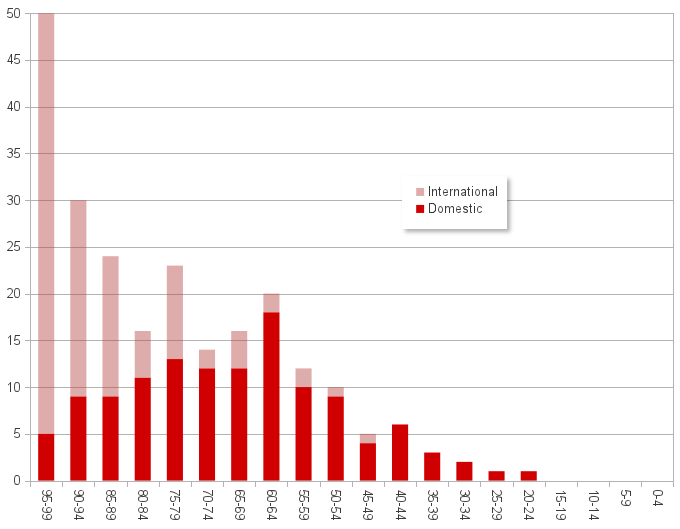
\includegraphics[width=.7\linewidth]{gre-math-percentiles}
\end{center}
\end{frame}

\begin{frame}{Percentiles}
\begin{center}
\begin{tabular}{cc}
Score | Percentile \\
\hline
960   | 96\\
880   | 90\\
840   | 82\\
780   | 70\\
740   | 62\\
680   | 50\\
640   | 42\\
580   | 30\\
\end{tabular}
\end{center}
\end{frame}

\begin{frame}{Resources}
\begin{itemize}
\item Princeton Review book
\item 5 official practice tests (found online)
\item \url{https://sites.math.rutgers.edu/~iacoley/greprep.html}
\item \url{https://www.varsitytutors.com/gre_subject_test_math-practice-tests}
\item google around!
\end{itemize}
\end{frame}

\begin{frame}{Strategy}
\begin{itemize}
\item The first 10-15 problems should be fast / easy
\item Try to do easiest problems in your head!
\item Harder problems: when we have to put pen to paper (toward middle)
\item Harder-er problems: linear algebra, abstract algebra (mixed in everywhere)
\item Hardest problems: special topics (towards the back)
\end{itemize}
\end{frame}

\section{Problems}

\subsection{Easy problems}

\begin{frame}{Problem 1}
$$\lim_{x\rightarrow 0}\frac{\sin(4x)-4x}{x^3}$$
\end{frame}

\begin{frame}{Problem 2}
Calculate
$$\int_{e^2}^{e^5} \frac{1}{x\log^2 x}$$
\end{frame}

\begin{frame}{Problem 3}
What is the value of the sum
$$\sum_{n=1}^\infty \frac{n^2+2}{n^3+3n + 5}$$
\end{frame}

\begin{frame}{Problem 4}
For which value of $a$ is 
$$\int_a^{a+1} (x^2+x) dx$$
a minimum?
\end{frame}

\begin{frame}{Problem 5}
If $V$ and $W$ are $5$-dimensional subspaces of $\mathbb{R}^7$, what can the dimension of $V\cap W$ be?
\end{frame}

\begin{frame}{Problem 6}
What is the greatest possible area of a triangular region with one vertex at the center of a circle of radius 1 and
the other two vertices on the circle?
\end{frame}

\subsection{Medium problems}


\begin{frame}{Problem 1}
Compute the second derivative of
 $$x^{x^x}$$
\end{frame}

\begin{frame}{Problem 2}
Compute
$$\lim_{n\rightarrow\infty} \frac{5}{n}\sum_{i=1}^n\left[\left(\frac{2i}{n}\right)^5-\left(\frac{2i}{n}\right)^3\right]$$
\end{frame}

\end{document}


